\documentclass[twocolumn]{article}

\usepackage{graphicx}
\usepackage{xeCJK}
\usepackage{bm}
\usepackage{amsmath,amsthm,amssymb,amsfonts}
\usepackage{cite}
\usepackage[colorlinks,linkcolor=red,anchorcolor=blue,citecolor=green,CJKbookmarks=true]{hyperref}
\usepackage{indentfirst}
\usepackage{amsmath}
\usepackage[margin=3.5cm]{geometry}
\usepackage{titlesec}
\usepackage{amsmath}
\usepackage{amssymb}
% \linespread{1.6}
\usepackage{multirow}
\usepackage{listings}
\usepackage{xcolor}
\usepackage{ulem}
\geometry{left=1.8cm,right=1.8cm,top=1.5cm,bottom=1.5cm}
\usepackage{enumitem}
\usepackage{tikz}
\usepackage{lipsum}
\setenumerate[1]{itemsep=0pt,partopsep=0pt,parsep=\parskip,topsep=5pt}
\setitemize[1]{itemsep=0pt,partopsep=0pt,parsep=\parskip,topsep=5pt}
\setdescription{itemsep=0pt,partopsep=0pt,parsep=\parskip,topsep=5pt}
%定理
\makeatletter
\thm@headfont{\sc}
\makeatother
\newtheorem{theorem}{Theorem}
%%%%%%%%%%%%% C++ Code
\usepackage{color}
\usepackage{xcolor}
\definecolor{keywordcolor}{rgb}{0.8,0.1,0.5}
\usepackage{listings}
\lstset{breaklines}%这条命令可以让LaTeX自动将长的代码行换行排版
\lstset{extendedchars=false}%这一条命令可以解决代码跨页时,章节标题,页眉等汉字不显示的问题
\lstset{ %用于设置语言为C++
    keywordstyle=\color{keywordcolor} \bfseries, 
    %identifierstyle=,
    basicstyle=\ttfamily, 
    commentstyle=\color{blue} \textit,
    stringstyle=\ttfamily, 
    showstringspaces=false,
    frame=shadowbox, %边框
    %captionpos=b
}

%\setCJKmainfont[BoldFont = 黑体]{宋体}
\setlength{\parindent}{2em}
%如果不要缩进 用\noindent
\title{\textbf{An Implementation of SAT-Based Two-Terminal \\ Path Finding Using Z3 Solver}}

\author{YiHong Gu \\ Tsinghua University \\ Beijing, China \\ gyh15@mails.tsinghua.edu.cn}

\date{}

\begin{document}

\maketitle

\section{Introduction}

The 'Two-Terminal Path Finding Problem' has the following description: given $N \times N$ routing grids, and $M$ pairs of terminals, you should use program to find routing paths connecting each pair of terminals. The limit is that different paths cannot cross each other, and no path can cross obstacles. The objective is to maxmize the number of connected pairs, and when all pairs of terminals can be connected, you should minimize the total length of all the paths.

In order to make the objective more clear and not change the original idea of the problem, we simply make the following stipulates that if one grid is defined to be one terminal of pair $d$, then other pairs $d'(d \neq d')$ can not route across the grid.

\section{Related Work}

\cite{source1} gives a general routing methodology which mainly uses 3 kinds of variable as parameters and use Z3 solver to solve the problem. The abstract idea is that giving a concrete illustration of each pairs: for each pair, define a droplet that starts from the origin and ends in terminal during time $t^*$ and $t^\dagger$, and then define the binary variable $c_{p,d}^t$ to illustrate whether the droplet $d$ is at the position $p$ in time $t$. It sets a lot of limits to ensure that (1) each droplet $d$ appears in the board during time $t^*_d$ to time $t^\dagger_d$ and it is at its origin position $p^*_d$ in time $t^*_d$ and at its terminal position $p^\dagger_d$ in time $t^\dagger_d$ (2) every second each droplet only appears at one position (3) the droplet satisfy the routing rule that can only step to one adjacent position per second.

Z3 solver\cite{source2}, developed by Microsoft Research, can use optimized algorithm to check whether it can satisfy all constraints and give a concrete solution. Moreover, it can also maximize/minimize one single variable or expression under all constraints.

\section{SAT-Based Model}

This part is divided into three main parts, sperately illustrate three different models: the original model which resembles the model established in\cite{source1}, the model which resembles network flow, the model which combined the 2 models above.

In the beginning, we just emphasize the definitions:

\begin{itemize}
	\item $N$: the size of the routing boards.
	\item $M$: number of pairs.
	\item $d$: the index of one single droplet.
	\item $t$: the time.
	\item $p$: one single position, can be represented by $p = (x, y) \in \{1, \cdots, N\} \times \{1, \cdots, N\}$.
	\item $P$: the set of all $p$.
	\item $B(p)$: the set of positions that are adjacent to the position $p$ in four direction(up, down, left, right).
	\item $p^*_d$, $p^\dagger_d$: the origin and terminal of droplet $d$.
\end{itemize}

\subsection{Model 1: Based on the Paper}

We use the notation that resembles the original notation in \cite{source1}, and define the binary variable $c_{p,d}^t$ to illustrate whether the droplet $d$ is at the position $p$ in time $t$, and the constraints can be divided into four main parts:

\textbf{to be or not to be}: we can simplify the $t^*$ and $t^\dagger$ and assume every droplet appears at the board in time $1$ (if we want to connect the two-terminal pair), so the constraints can be (for each $d$):

\[
 c_{p^*_d,d}^1 \to \bigvee_{t=1}^{T} c_{p^*_d, d}^t
\]

It means: if it appears, then it must reach the terminal.

\textbf{second conflict}: it means every second each droplet only appears at one position, so the constraints can be (for each $d$):

\[
\bigwedge_{t=1}^{T} \bigwedge_{p \in P} \bigwedge_{p' \in P, p' \neq p} \neg c_{p, d}^t \vee \neg c_{p', d}^t
\]

\textbf{position conflict} firstly every grid can only be visited once (for each $p$)

\[
\bigwedge_{d=1}^{M} \bigwedge_{d'=d+1}^{M} \bigwedge_{t=1}^{T}  \bigwedge_{t'=t+1}^{T} \neg c_{p, d}^t \vee \neg c_{p, d'}^{t'}
\]

\[
\bigwedge_{d=1}^{M} \bigwedge_{t=1}^{T}  \bigwedge_{t'=t+1}^{T} \neg c_{p, d}^t \vee \neg c_{p, d}^{t'}
\]

Also, for each position $p$ which has obstacles for droplet $d$, for all $t$, $c_{p, d}^t$ must be FALSE.

\textbf{travel constraints}: it means the droplet satisfy the routing rule that can only step to one adjacent position per second. So for each droplet $d$, if it appears at position $p$ in time $t$, it must appears at the adjacent position $p'$ in time $t-1$ (except $t=1$).

\[
c_{p, d}^t \to (\bigvee_{p' in B(p)} c_{p', d}^{t-1})
\]

\textbf{optimization object}: if we want to maxmize the total pairs, we just need to maxmize

\[
\sum_{d=1}^{M}{[c_{p^*_d,d}^1]}
\]

If we want to minmize the total length, we firstly enforce that every $c_{p^*_d,d}^1$ should be TRUE and then minimize

\[
\sum_{d}\sum_{p}\sum_{t}{[c_{p,d}^t]}
\]

Note that the notation

\[
[statement] = \begin{cases} 1, &statement = TRUE\cr 0, &statement = FALSE\end{cases}
\]

We can find the scale of the variables and the constraints are very large, we have totally $T \times N^2 \times M^2$ variables and almost $O(T^2 N^4 M^2)$ contraints, which $T$ represents the maximum time used and it can be $\frac{N^2}{2}$ under the worst condition. If we simply make $N$ be $10$, $M$ be $4$, we can't afford to work it out by our personal computer.

\subsection{Model 2: Based on the Network Flow}

In this model, we directly use the model resembles network flow architecture, for each droplet $d$, we build a network flow graph and set the source to be the origin and sink to be the terminal, and all the positions must satisfy the flow conservation. Then we have $M$ layers network flow graph, afterwards we implement the constraint that every position can be only visited once using a constraint like linear constraint.

In this model, if we use some artifice, we can only have totally $2 \times N^2 \times M$ variables and $O(\times N^2 \times M)$ contraints. Besides, after a large quantity of attempts we find if we conbine several contraints together, we can accelerate the speed of our algorithm, and this things can be concretely described in the next section.

\subsection{Model 3: The Mixed One}

Combine model 1 and model 2 together, we can find a more efficient model, which only have $N^2 \times M$ variables and is 1.5 times faster than model 2.

We use the binary variable $c_{p,d}$ to represent whether the droplet $d$ visit across the position $p$, therefore the contraints are as follows:

\textbf{limit terms} if it is a barrier or is not in the corresponding layer, we enforce $c_{p,d}$ to be FALSE, also we force that every position can only be visited once by the following contraint (for each $p$)

\[
\sum_{d=1}^{M} [c_{p,d}] \le 1
\]

\textbf{source and sink terms}: for each $d$, we come up with a contraint that

\[
c_{p^*_d,d} \leftrightarrow c_{p^\dagger_d,d}
\]

\textbf{connection terms}: for each $p$ which is not the terminal/origin/obstacle grid, it must satisfy the following contraint for each $d$:

\[
c_{p,d} \to (\sum_{p' \in B(p)}c_{p',d} = 2)
\]

and for each $p$ which is equal to $p^*_d$ or $p^\dagger_d$ for a specific $d$, it must satisfy the following contraint:

\[
c_{p,d} \to (\sum_{p' \in B(p)}c_{p',d} = 1)
\]

\textbf{optimization object}: if we want to maxmize the total pairs, we just need to maxmize

\[
\sum_{d=1}^{M}{[c_{p^*_d,d}]}
\]

If we want to minmize the total length, we firstly enforce that every $c_{p^*_d,d}$ should be TRUE and then minimize

\[
\sum_{d}\sum_{p}{[c_{p,d}]}
\]

\section{Optimization}

However, the models above don't have efficiency when the graph is sparse. For example, for a board that $N=10$, if we set $M=9$ and place the 9 pairs over the whole board, it runs quite fast (about 1.5 second, model 2), but if we set $M=2$ and place the 2 pairs like the following Figure\ref{aee}, it takes almost 30 minutes to get the best answer.

\begin{figure}
    \centering
    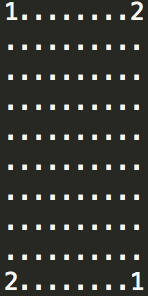
\includegraphics[height = 3cm]{example}
    \caption{An Extreme Example}
    \label{aee}
\end{figure}

\newpage

In order to optimize the algorithm, we come up with three main points:

(1) We can combine some muti-SAT terms together to a mixed term, which can reduce the check time (it can approximately accelerate the speed twice).

(2) It has no meaning if one droplet $d$ takes the squared area, it means the situation

\[
c_{p_1, d} = c_{p_2, d} = c_{p_3, d} = c_{p_4, d} = TRUE
\]

should be forbidden where $p_1 = (x, y)$, $p_2 = (x + 1, y)$, $p_2 = (x, y + 1)$, $p_4 = (x + 1, y + 1)$, Z3 solver will search all the posibilities including this situation. But, under the circumstances of this specific problem, this situation don't contribute any to the final answer. Therefore, we can manually add the \textbf{prune term 1} for each $p$ and $d$ (where $p_1 = p$):

\[
\neg(c_{p_1, d} \wedge c_{p_2, d} \wedge c_{p_3, d} \wedge c_{p_4, d})
\]

(3) when consider the 4 totally empty grid (no obstacle/terminal), for one single droplet, there are 2 ways to pass from the left-down to up-right, just like the Figure \ref{a4v}.

\begin{figure}
    \centering
    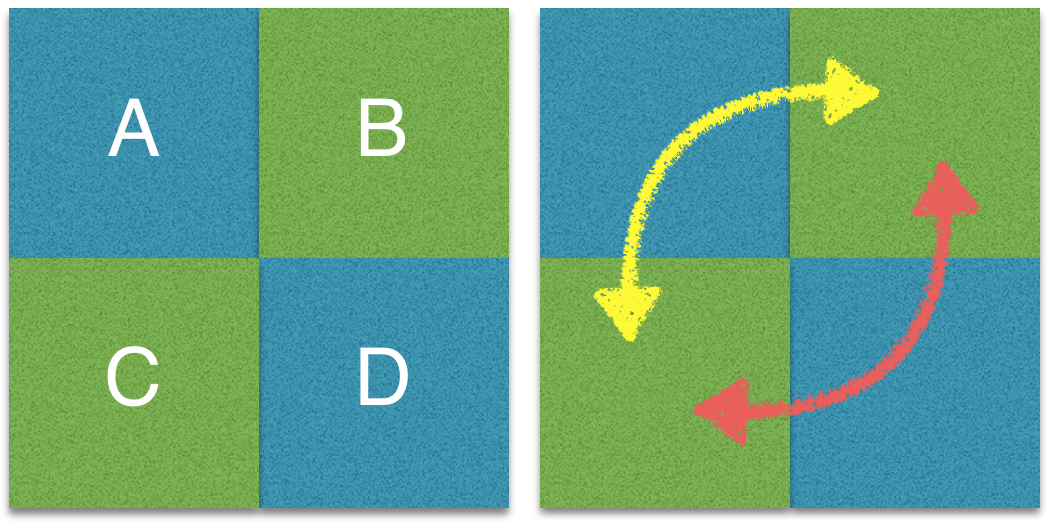
\includegraphics[height = 3cm]{example2}
    \caption{A 4-Block View}
    \label{a4v}
\end{figure}

we can find the path C-A-B and C-D-B are both ok, and Z3 solver will check all the 2 path, so we can forbid this situation simply by the following contraint \textbf{prune term 2}(we forbid C-D-B for any $p$ and $d$):

\[
(\sum_{x=1}^{M}{[c_{p_1,x}]} = 0) \to \neg(c_{p_2,d} \wedge c_{p_3,d} \wedge c_{p_4,d})
\]

where $p = p_1 = (x, y)$, $p_2 = (x + 1, y)$, $p_2 = (x, y + 1)$, $p_4 = (x + 1, y + 1)$. Moreover, we can strength the contraint by the following expression if we check other conditions.

\[
(\sum_{x=1}^{M}{[c_{p_1,x}]} = 0) \to \neg(c_{p_2,d} \wedge c_{p_3,d})
\]

and another symmetric terms should also be added (to forbid A-C-D from 2 paths A-C-D and A-B-D)

The prune term 1 and prune term 2 is of great significance, if we use these terms, we can get the answer of example in Figure \ref{aee} in 1.5 seconds.

\section{Results and Evaluation}


\section{System Architecture}

\section{GUI}

\section{Conclusions}

\begin{thebibliography}{1}
\bibitem{source1}
Oliver Keszocze, Robert Wille, Krishnendu Chakrabarty, Rolf Drechsler. A General and Exact Routing Methodology for Digital Microfluidic Biochips.
\bibitem{source2}
Leonardo De Moura and Nikolaj Bjørner. Z3: An efficient SMT solver. In Tools and Algorithms for the Construction and Analy- sis of Systems, pages 337–340. Springer, 2008. Z3 is available at http://z3.codeplex.com/.
\end{thebibliography}


\end{document}

